\debut{Emile Martinez}{Lycée}{Aucun}{Tannenbaum, Balabonski 1ère}

\section{Modèle Client-Serveur}

\subsection{Le modèle}

\begin{definition}[Client/Serveur]
	Dans un réseau informatique, les échanges de données entre deux ordinateurs sont souvent asymétriques. Un ordinateur, désigné comme le client, demande généralement des ressources (des données) à un autre ordinateur, appelé serveur, qui les fournit à tous ceux qui en font la demande.
\end{definition}

\begin{example}
	En tapant «http://www.google.fr», votre machine va chercher à entrer en communication avec le serveur portant le nom «google.fr». Votre machine est ici client.
\end{example}

\begin{rem}
	N'importe quel type d'ordinateur peut jouer le rôle de serveur, mais dans le monde professionnel les serveurs sont des machines spécialisées conçues pour fonctionner 24h sur 24h.
\end{rem}

\begin{personalise}[Schéma] \\
	\label{25-modele}
	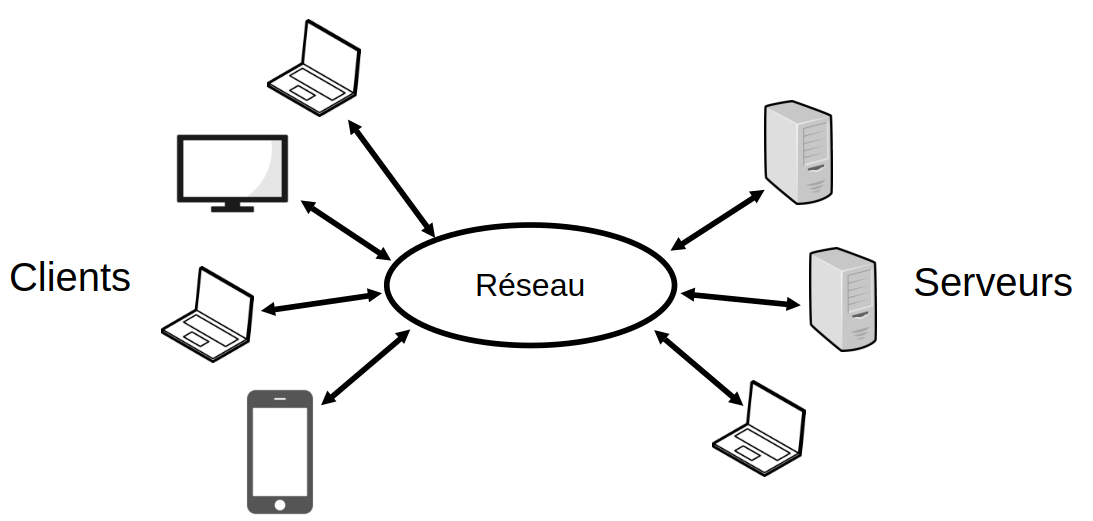
\includegraphics[width=0.7\linewidth]{lecon/25-client-serveur/modele.png}
\end{personalise}

\begin{rem}
	Un même ordinateur peut être à la fois plusieurs clients et plusieurs serveur 
\end{rem}

\begin{rem}
	Dans ce modèle les clients ne communiquent pas entre eux (ni les serveurs entre eux). Seuls des clients communiquent avec des serveurs
\end{rem}

\subsection{Caractéristiques concrètes}

\begin{principe}
	Caractéristiques d'un serveur : \begin{itemize}[label=$\star$]
		\item Son adresse IP est permanente, et le serveur attend une connexion entrante sur un ou plusieurs ports. On dit qu'il écoute.
		\item A la connexion d'un client sur le port en écoute, il ouvre une socket (interface de connexion)\footnote{traduction proposée par wikipédia, mais qui ne semble pas universellement admise}. Il n'est pas à l'initiative de la connexion
		\item A la suite de la connexion, le processus serveur communique avec le client suivant un protocole établi préalablement. L'action réalisée par le serveur en réponse à la requête client est souvent appelée service.
	\end{itemize}
\end{principe}

\begin{principe}
	Caractéristiques d'un client : \begin{itemize}
		\item Il est à l'initiative de l'établissement la connexion avec le serveur
		\item Lorsque la connexion est acceptée par le serveur, il communique comme le prévoit la couche application du modèle OSI
	\end{itemize}
\end{principe}

\begin{com}
	Bon ces deux caractérisations demandent à être améliorées, et éventuellement élaguées. De plus, on peut se poser la question si pour bien expliquer que ce n'est pas en tant que tel une machine qui est client ou serveur, mais une application/un programme, on pourrait pas mettre «caractéristiques d'un programme serveur /client». Mais un client pouvant être plus qu'un programme \dots. Tout cela demande réflexion.
\end{com}

Le protocole d'échange se divise alors ici en deux couches : la couche transport et la couche application.

\begin{definition}[Couche transport]
	 C'est le trait de la machine vers le réseau dans le schéma \ref{25-modele}. C'est le protocole qui met sur le réseau les données et qui les en récupèrent. (ex : TCP, UDP)
\end{definition}

\begin{definition}[Couche application]
	C'est la manière de choisir quelle données on veut échanger et de quelle manière on les envoie. Par analogie, choisir un protocole applicatif, c'est comme choisir une langue dans laquelle communiquer.
\end{definition}

\subsection{Est-ce tout internet ?}

Vous avez peut-êre entendu parler de protocole pair-à-pair, sans serveurs, et où les données s'échangent entre clients

\begin{personalise}[Schéma]\\
	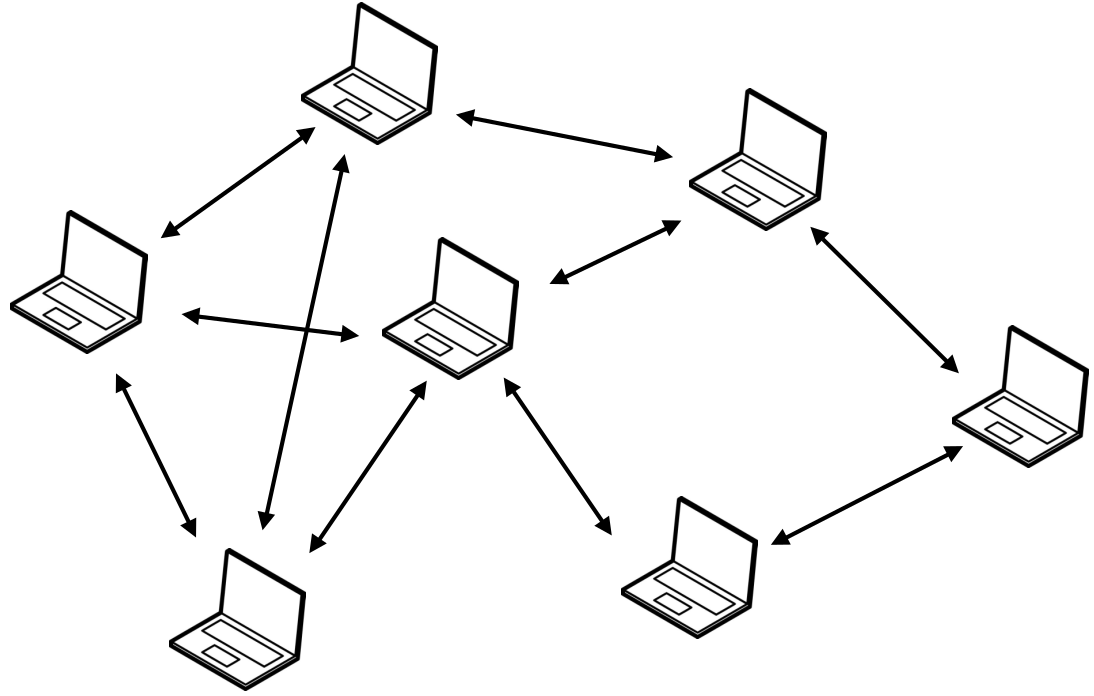
\includegraphics[width=0.5\linewidth]{lecon/25-client-serveur/pair-a-pair.png}
\end{personalise}

En réalité, nous sommes encore dans le modèle client serveur. En effet, chaque client joue alternativement le rôle de client et de serveur.

\begin{rem}
	L'ancien modèle de communication téléphonique fonctionnait en connectant directement les deux hôtes via un canal qui leur était réservé.
\end{rem}

\section{La couche transport}

\subsection{Introduction}

\begin{definition}[numéro de port]
	Les protocoles de transport définissent un numéro de port, c'est à dire un identifiant numérique associé à une application particulière. Il permet à une même machine d'établir plusieurs communication réseau en parallèle.
\end{definition}

\begin{example}
	Le numéro de port par défaut pour le web non sûr (protocole HTTP) est le 80, et celui pour le web sécurisé (HTTPS) est le 443. Ce ne sont cependant que des conventions, un serveur web peut attendre des connexions sur un autre port.
\end{example}

\begin{principe}[Principe de Segmentation]
	Plutôt que d'envoyer toutes les données d'un seul tenant, la couche transport les découpe en plein de paquets plus petits qu'on envoie séparemment.\end{principe}
\begin{personalise}[Intérêts] \begin{itemize}[label=$\star$]
		\item Plusieurs paquets peuvent cohabiter sur un même lien (plus équitables)
		\item En cas de paquet perdu ou corrompu, on peut ne renvoyer que le paquet en question (et pas tout le message)
		\item On peut exploiter la redondance des liens du réseau en faisant emprunter plusieurs chemin à différents paquets
	\end{itemize}
\end{personalise}

\begin{principe}[Principe d'encapsulation]
	Chaque couche du réseau ajoute un en-tête aux données que l'on envoie, et considère les données d'un bloc (sans différencier les données d'éventuels en-tête de couches précédentes).\begin{center}
		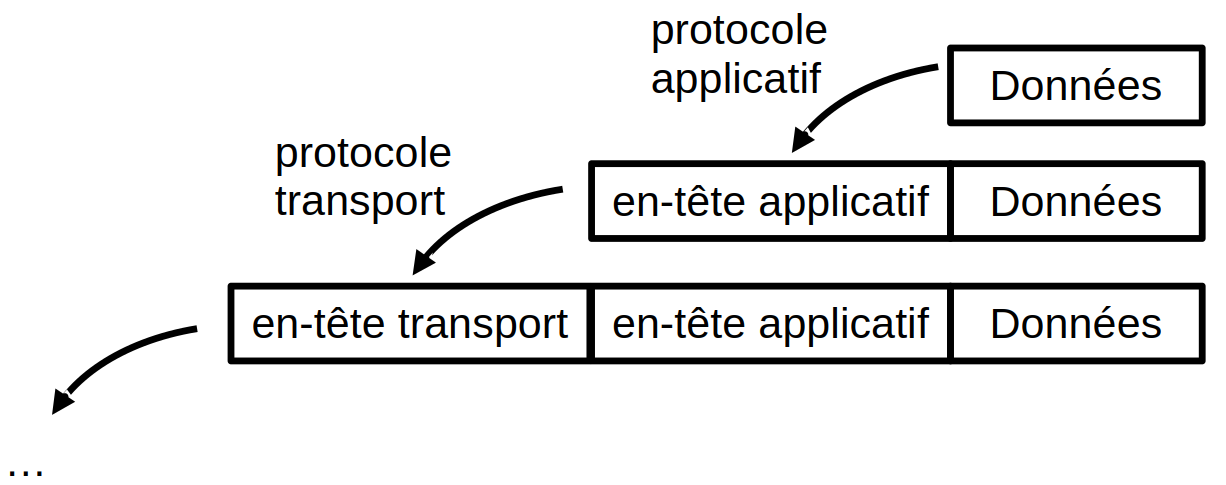
\includegraphics[width=0.6\linewidth]{lecon/25-client-serveur/encapsulation.png}
	\end{center}
\end{principe}

\subsection{Le protocole TCP}

\begin{principe}
	\label{25-tcp}
	Le protocole TCP permet, après l'initialisation d'une connexion, d'envoyer des données de taille arbitraire, dans l'ordre, de détecter les erreurs de transmission et de retransmettre les fragments de données perdus ou corrompus.
\end{principe}

\paragraph{Étape 1 :} Connexion en 3 temps\\
\begin{minipage}{0.4\linewidth}
	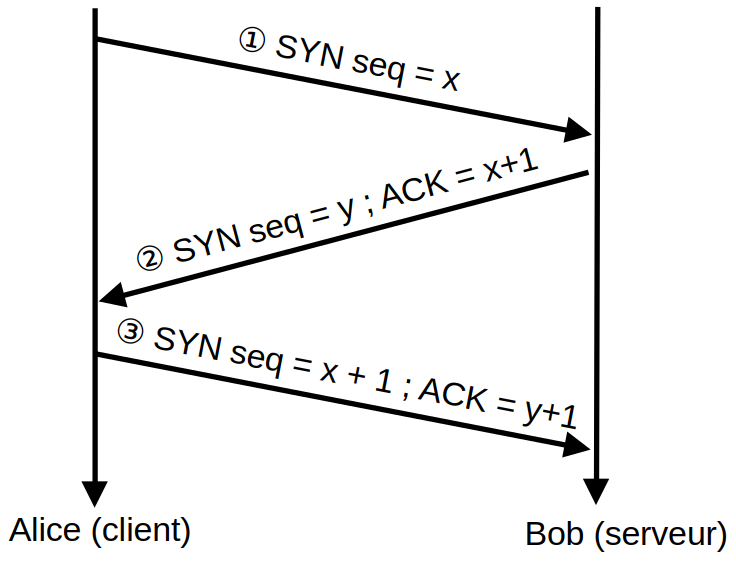
\includegraphics[width=\linewidth]{lecon/25-client-serveur/3-temps.png}
\end{minipage} \quad\begin{minipage}{0.55\linewidth}
	\begin{itemize}
		\item[$\circled{1}$] Le client choisit un numéro de séquence aléatoire et envoie un paquet SYN (pour synchronisation) indiquant ce numéro
		\item[$\circled{2}$] Le serveur reçoit le paquet et choisit un autre numéro aléatoire et renvoie un paquet SYN - ACK (synchronized - acknowledgment) contenant le numéro de séquence du client incrémenté de 1 et son propre numéro de séquence.
		\item[$\circled{3}$] Le client reçoit le paquet. Il est considéré comme connecté ! Il envoie «bien reçu» grâce au paquet ACK y+1
	\end{itemize}
	A la reception de ce paquet, le serveur est connecté
\end{minipage}

\paragraph{Étape 2 :} Transfert de données et retransmission\\
\begin{minipage}{0.4\linewidth}
	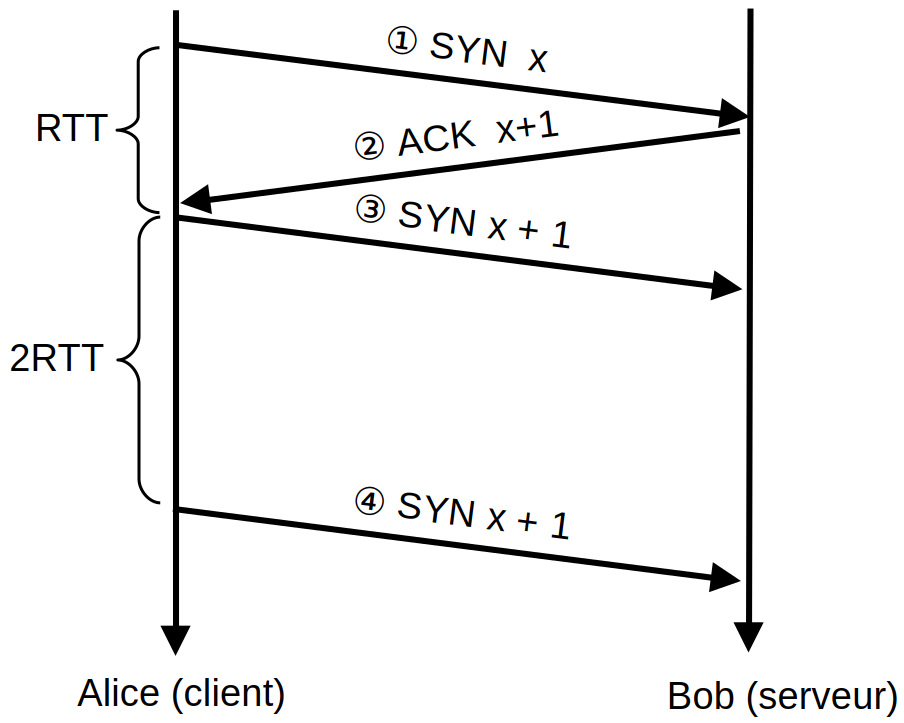
\includegraphics[width=\linewidth]{lecon/25-client-serveur/transfert-tcp.png}
\end{minipage} \quad \begin{minipage}{0.55\linewidth}
	\begin{itemize}
		\item[$\circled{1}$] Alice envoie un paquet de données identifié par un numéro de séquence.
		\item[$\circled{2}$] Bob le reçoit et indique la bonne réception avec un paquet ACK
		\item[$\circled{3}$] Alice n'a toujours pas reçu le ACK après 2 RTT = 2 fois le temps moyen d'un aller retour. Elle renvoie le paquet.
	\end{itemize}
\end{minipage}

\begin{rem}
	Les numéros de séquences nous permettent d'envoyer le paquet suivants avant d'avoir reçu l'acquittement du précédent, tout en restant fiable (cf. principe \ref{25-tcp}) (car on sait alors les remettre dans l'ordre, et à quel paquet correspond un acquittement).
\end{rem}

\paragraph{Développement :} La fenêtre glissante dans le protocole TCP pour augmenter le taux d'envoi et éviter la congestion.

\subsection{Socket TCP en Python}

\begin{definition}
	Une socket est une interface logicielle, c'est à dire un objet qui représente le bout de la connexion entre deux machines.
\end{definition}

\begin{algo}
	\begin{lstlisting}[style=PythonStyle]
# serveur TCP python
from socket import socket 
serveur = socket() #creation de la socket
serveur.bind(('0.0.0.0', 9999)) #port 9999
serveur.listen()
while True :
    #sclient : socket du client, adclient : addresse IP du client
    (sclient, adclient) = serveur.accept()
    # On attend que le client lui envoie au moins 1000 octets de données
    donnees = sclient.recv(1000)
    while donnees : 
        #traitement
        donnees = sclient.recv(1000)
    sclient.close()
	\end{lstlisting}
	\begin{lstlisting}[style=PythonStyle]
# client TCP python
from socket import socket
serveur = socket()
serveur.connect('127.0.0.1', 9999) #IP et port du serveur auquel se connecter
phrase = input()
while phrase != 'FIN':
	phrase = phrase + '\n'
	serveur.send(phrase.encode())
	phrase = input()
	\end{lstlisting}
\end{algo}

\section{La couche application}

Quand un client souhaite accéder à une page web, il tape un URL (ex : http://wikipedia.fr/informatique) dans la barre du navigateur web. Cette URL se découpe en 3 morceaux : \begin{itemize}
	\item http ou https qui précise le protocole de la couche application utilisé
	\item le nom de domaine (ex : wikipedia.fr) ou l'adresse IP du serveur
	\item le document demandé au serveur (ex : la page informatique du serveur wikipedia) 
\end{itemize}

\subsection{Le protocole HTTP (Hypertext transfer protocol)}

\begin{definition}
	Le protocole HTTP est un protocole applicatif qui définit les messages envoyés entre le navigateur (client) et le serveur. Les messages envoyés par le client sont des requêtes, ceux envoyés par le serveur des réponses. 
\end{definition}

\begin{definition}[méthode]
	Les requêtes d'un client commence par un mot clef qui indique la méthode utilisée, c'est à dire la nature du message envoyé. Les méthodes les plus communes sont GET, HEAD et POST.
\end{definition}

\begin{itemize}[label=$\star$]
	\item GET : Demande une ressource sans la modifier. C'est la méthode la plus courante pour demander d'afficher une page web par exemple
	\item POST : transmet une donnée (ex: envoi de forumlaire)
	\item HEAD : Cette méthode ne demande que des informations sur la ressource, sans demander la ressource elle-même
\end{itemize}

\begin{example}[navigation vers l'URL http://wikipedia.fr/informatique]
	Le client envoie la requête
	\begin{lstlisting}
GET /informatique HTTP/1.1
Host : www.wikipedia.fr
	\end{lstlisting}
	qui anonnce au serveur (wikipedia) que l'on utilise HTTP en version 1.1 pour obtenir la ressource informatique de wikipedia.\\
	
	Le serveur répond alors
	\begin{lstlisting}
HTTP/1.1 200 OK #accepte de communiquer et de transmettre la ressource
Serveur: wikipedia.fr
Date: 27.07.1214
Content-Type: text/html

<html class ="client...
<@et le reste de la page wikipedia visible à \url{view-source:https://fr.wikipedia.org/wiki/Informatique}@>
	\end{lstlisting}
	Si jamais la ressource demandée n'existe pas ou est indisponible, la réponse sera
	\begin{lstlisting}
HTTP/1.1 404 Not Found #ressource non trouvée
Server: wikipedia.fr
Date: 27.07.1214
Content-type:
<@suivi de la page html décrivant l'erreur@>
	\end{lstlisting}
\end{example}

\subsection{HTTPS}

Le protocole HTTP est clair : si une personne intercepte les paquets de données sur le réseau entre un client et un serveur, elle peut lire le contenu des messages échangés, par exemple des mots de passe confidentiels. Le protocole HTTPS fonctionne comme le protocole HTTP, mais en chiffrant les messages. 

\paragraph{Développement :} Le S du protocole HTTPS : authentification et chiffrement des messages.

